\documentclass[10pt]{article}

\usepackage[letterpaper,margin=0.72in,columnsep=0.26in]{geometry}
\usepackage{amsmath,amssymb,bm,mathtools}
\usepackage{booktabs}
\usepackage{array}
\usepackage{microtype}
\usepackage{setspace}
\usepackage{enumitem}
\usepackage[hidelinks]{hyperref}
\usepackage{xcolor}
\usepackage{siunitx}
\usepackage{caption}
\usepackage{balance}
\usepackage{tikz}
\usepackage{pgfplots}
\usetikzlibrary{arrows.meta,positioning,calc}
\pgfplotsset{compat=1.18}

\setstretch{1.08}
\setlength{\parindent}{1.15em}
\setlength{\parskip}{0.18em}
\setlist{nosep,leftmargin=*}
\captionsetup{font=small,labelfont=bf}
\sisetup{detect-all=true}
\raggedbottom
\setlength{\emergencystretch}{2em}

\newcommand{\TEF}{\mathrm{TEF}}
\newcommand{\dd}{\mathrm{d}}
\newcommand{\ii}{\mathrm{i}}
\newcommand{\conceptbox}[1]{\begin{center}\fbox{\parbox{0.91\columnwidth}{\centering #1}}\end{center}}
\providecommand{\tightlist}{\setlength{\itemsep}{0pt}\setlength{\parskip}{0pt}}

\hypersetup{
  pdftitle={The Emergent Frame: A Minimal Framework for Spacetime Rollout, Interaction, and Excitation},
  pdfauthor={Xiaodan Wu},
  pdfsubject={The Emergent Frame; spacetime rollout; matter topology; spacetime excitation; emergent gravity},
  pdfkeywords={The Emergent Frame, emergent spacetime, spacetime rollout, helical spacetime, matter topology, matter-spacetime interface, phase transport, gauge connection, emergent gravity, topological matter, confinement},
  pdfproducer={LaTeX},
  pdfcreator={Xiaodan Wu},
  pdfinfo={DOI={10.5281/zenodo.22723329}}
}

\title{\bfseries The Emergent Frame:\\
A Minimal Framework for Spacetime Rollout, Interaction, and Excitation}
\author{\small Xiaodan Wu\textsuperscript{1,*}\\
\footnotesize \textsuperscript{1}Independent Researcher\textsuperscript{\(\dagger\)}}
\date{\footnotesize September 12, 2026 --- Version 2.5}

\begin{document}
\twocolumn[
\begin{@twocolumnfalse}
\maketitle
\vspace{-0.7em}
\begingroup
\normalsize
\setstretch{1.08}
\begin{center}
\textbf{Abstract}
\end{center}
\noindent
The Emergent Frame (TEF) explores whether the physical spacetime frame associated with matter may itself be emergent. Earlier studies investigated helical spacetime geometry, persistent matter topology, closure energetics, and matter--spacetime interface constructions. This paper brings these strands together into a compact working framework for spacetime rollout, interaction, and excitation.

The proposed picture distinguishes persistent closed matter topology, the spacetime structure it continuously updates through rollout, and excitation modes supported by that structure. Globally complete matter closures are provisionally assigned independent rollout-source identity, while excitations are not; nevertheless, the full energy--momentum state must still contribute to gravitational backreaction. The inherited helix provides a local geometric realization in which transverse phase closes while axial advance continues, without by itself constituting a wave dynamics.

Photon and electron phenomena are investigated as different excitation classes, with rollout supplying a possible local phase reference and transport structure while quantum excitations retain state-dependent phase and internal degrees of freedom. Interaction is approached through structural compatibility: strong-sector phenomena motivate closure energetics, matter-changing weak processes motivate interface reconfiguration, electromagnetism motivates covariant phase transport, and gravity motivates compatibility between matter-associated rollouts. These are research directions rather than completed interaction laws.

A separate empirical relation yields a candidate closure scale of $444.56\,\mathrm{MeV}$, retrospectively close to a reported lattice-QCD flux-tube scale. It is retained only as a calibration conjecture.

The paper establishes a working baseline for subsequent dynamical constructions and explicit tests.

\vspace{0.65em}
\noindent\textbf{Keywords:} emergent spacetime; spacetime rollout; helical spacetime; matter topology; matter--spacetime interface; phase transport; gauge connection; emergent gravity; topological matter; confinement.
\endgroup

\vspace{1.65em}
\end{@twocolumnfalse}
]
\begingroup
\renewcommand{\thefootnote}{\fnsymbol{footnote}}
\footnotetext[1]{\href{mailto:xiaodan@theemergentframe.org}{xiaodan@theemergentframe.org}}
\footnotetext[2]{\href{https://theemergentframe.org}{https://theemergentframe.org}; ORCID: 0009-0005-5892-0293; DOI: \href{https://doi.org/10.5281/zenodo.22723329}{10.5281/zenodo.22723329}.}
\endgroup
\section{\texorpdfstring{Why \emph{The Emergent Frame}?}{Why The Emergent Frame?}}\label{why-the-emergent-frame}

The name \emph{The Emergent Frame} came before most of the present machinery.

Special relativity teaches that measured lengths and durations are not universal quantities independent of physical state and relative motion. Conventionally, \[
\gamma=\frac{1}{\sqrt{1-v^2/c^2}},
\qquad
\Delta t=\gamma\Delta\tau,
\qquad
L=\frac{L_0}{\gamma}.
\]

Within standard relativity these relations follow from Minkowski geometry. TEF does not dispute that description. The motivating question is more primitive:

\begin{quote}
If operational spatial and temporal scales are inseparable from physical state and motion, is the frame itself necessarily a pre-existing stage?
\end{quote}

TEF explores the alternative possibility that the physically realized spacetime frame associated with matter is generated or continuously updated by matter.

This is a reverse-engineering programme. Established experimental physics is treated as specification rather than something to be discarded. The aim is to ask whether a smaller set of geometric and topological primitives can reproduce structures that are presently taken as independent inputs.

TEF belongs to a broader family of approaches in which spacetime geometry is not necessarily treated as the final microscopic primitive. Jacobson showed that the Einstein equation can be read as an equation of state emerging from local horizon thermodynamics \cite{Jacobson1995}. Spinor-gravity programmes have explored the possibility that vielbein and metric variables arise as composite objects built from more fundamental spinorial degrees of freedom \cite{Wetterich2004}. Causal fermion systems provide a different relational construction in which spacetime is described through correlations of a many-body quantum system \cite{FischerPaganini2026}. These approaches do not imply TEF and are not used here as evidence for its specific ontology. They locate the problem class: TEF differs by assigning a distinctive role to persistent matter closure, matter-associated spacetime rollout, and excitation on the resulting frame.

Paper I \cite{WuPaperI} introduced a gravity-calibrated primitive radius \[
R=\frac{\ell_P}{2},
\] together with a frozen dimensionless helical shape parameter \(q\) satisfying \[
q\sqrt{1+q^2}=\frac{2}{\pi}.
\]

Papers II \cite{WuPaperII} and III \cite{WuPaperIII} tested the same frozen geometry against additional cross-sector correspondences. Paper IV \cite{WuPaperIV} then changed emphasis: open spacetime was treated geometrically, while persistent matter was investigated through topology, relative framing, and closure. Paper V \cite{WuPaperV} developed the closure branch toward confinement energetics. Paper VI then investigated matter--spacetime interface constructions \cite{WuPaperVI}, asking how matter and open spacetime might couple without assuming that they are globally the same object.

The purpose of the present paper is to reconnect those branches into one narrative. It does not claim that a completed unified dynamics has already been obtained.

\section{Where TEF Begins---and Where It Stops}\label{where-tef-beginsand-where-it-stops}

TEF does not attempt to identify the ultimate substrate of existence.

Matter topology, spacetime rollout, quantum excitation, vacuum fluctuation, annihilation, and pair creation may all ultimately be manifestations of a deeper level. Human theories may call that level vacuum, quantum vacuum, field ground state, substrate, ether-like medium, or something else. A name does not establish that its ontology has been understood.

The present work therefore places a deliberate boundary below the modeled layer.

Within TEF, the three structural categories are

\conceptbox{closed matter topology \\ spacetime rollout \\ spacetime excitation}

The deeper substrate is outside scope.

This boundary is not a loophole. Observable formation, destruction, or reconfiguration of matter closures remains a TEF obligation because such changes alter the modeled source structure. Likewise, redistribution of energy and momentum among matter, radiation, and interactions must be accounted for at the effective level. What TEF declines to model is the ultimate ontological ``stuff'' beneath those observable structural changes.

Accordingly, the framework does not require a literal statement such as \[
\text{matter}\rightarrow\text{photon}
\] at the ontological level. It instead asks what happens, within the modeled layer, to closure, rollout-source identity, excitation state, and energy--momentum bookkeeping before and after the process.

\section{A Minimal Ontology of Matter and Rollout}\label{a-minimal-ontology-of-matter-and-rollout}

\subsection{Matter as persistent global closure}\label{matter-as-persistent-global-closure}

The present working hypothesis is

\conceptbox{Persistent matter corresponds to dynamically admissible global closure.}

Closure is a property of the whole admissible configuration, not necessarily of each locally identifiable segment.

This distinction is inherited from the matter-topology branch of TEF. A quark-like sub-sector may be locally persistent yet globally incomplete. By contrast, a hadron-like configuration may constitute a complete closure. More weakly bound systems may contain several independently complete closures without becoming a new primitive closure merely because they are bound.

The resulting hierarchy is:

\conceptbox{Only a level that is itself globally complete can possess independent rollout-source identity.}

This statement does not specify the microscopic shape of the closure. Paper IV deliberately kept that question open, and the present paper does the same.

\subsection{Rollout as structural update}\label{rollout-as-structural-update}

For a complete source \(C\), TEF writes schematically

\[
C:\quad S(t)\rightarrow S(t+dt).
\]

The word \emph{rollout} should not be read as ``matter emits something into an already existing empty volume.'' If spatial measure is itself emergent, then primitive rollout cannot be defined by dilution through a pre-existing area or volume.

The present interpretation is instead that matter continuously updates the realized spacetime structure associated with it.

A useful working hierarchy is

\conceptbox{phase-bearing rollout structure $\longrightarrow$ emergent spatial geometry and measure}

Consequently, statements such as ``the rollout becomes weaker because it spreads over \(4\pi r^2\)'' cannot be primitive explanations. The spatial measure and its radial scaling have first to emerge from the rollout geometry.

\subsection{An intrinsic source label}\label{an-intrinsic-source-label}

To discuss source strength without importing a pre-existing volume density, let

\[
\Phi_R(C)
\]

denote an intrinsic, boost-independent rollout-source label associated with a complete closure \(C\).

At this stage \(\Phi_R\) is intentionally underdefined. Its physical dimension, normalization, conservation law, discreteness, and relation to effective geometry have not been derived.

It should therefore not yet be called a conserved flux or an established gravitational charge.

The only current claim is narrower:

\conceptbox{$\Phi_R(C)$ is intended to label an intrinsic property of a complete closure, not an observer-dependent boost energy.}

Composite systems may later require interaction corrections, but until a dynamical law is supplied expressions such as \[
\Phi_R^{\rm system}
=
\sum_i\Phi_{R,i}
+
\Delta\Phi_{\rm int}
\] are bookkeeping ansätze rather than derived equations.

\section{Helical Rollout: Phase Closure Without a Wave Equation}\label{helical-rollout-phase-closure-without-a-wave-equation}

The geometric intuition inherited from Paper I is based on a circular helix,

\[
\mathbf r(\theta)
=
\bigl(a\theta,\;R\cos\theta,\;R\sin\theta\bigr),
\qquad
q=\frac{a}{R},
\]

where the dimensionless ratio \(q\) is the frozen helical shape parameter introduced in Paper I.

Viewed along the rollout axis, \[
(y,z)=(R\cos\theta,R\sin\theta),
\] so the transverse structure closes as \[
y^2+z^2=R^2.
\]

Viewed from the side, \[
x=a\theta,
\qquad
y=R\cos\theta,
\] and therefore \[
y=R\cos(x/a).
\]

After a complete phase cycle, \[
\theta\rightarrow\theta+2\pi,
\] the transverse phase returns to its initial value while the axial coordinate advances by \[
\Delta x=2\pi a.
\]

The compact geometric statement is therefore

\conceptbox{Phase closes while rollout continues.}

This picture is useful because circular phase rotation and longitudinal spatial periodicity are two projections of the same local geometry.


Figure~\ref{fig:helix-projections} summarizes these three views of the same local construction.

\begin{figure*}[t]
\centering
\begin{minipage}[t]{0.32\textwidth}
\centering
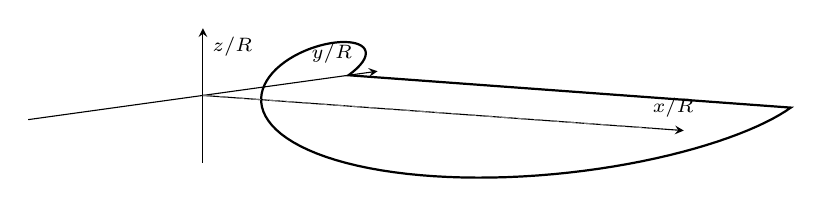
\begin{tikzpicture}
\begin{axis}[
    width=\linewidth,height=4.35cm,
    view={36}{24},
    axis lines=center,
    xlabel={$x/R$},ylabel={$y/R$},zlabel={$z/R$},
    xmin=0,xmax=3.8,ymin=-1.2,ymax=1.2,zmin=-1.2,zmax=1.2,
    ticks=none,
    clip=false,
    label style={font=\scriptsize},
]
\addplot3[black,thick,domain=0:360,samples=90]
({0.55632418*x*pi/180},{cos(x)},{sin(x)});
\addplot3[black!55,dashed] coordinates {(0,0,0) (3.55,0,0)};
\end{axis}
\end{tikzpicture}

\small (a) Local helical rollout
\end{minipage}\hfill
\begin{minipage}[t]{0.32\textwidth}
\centering
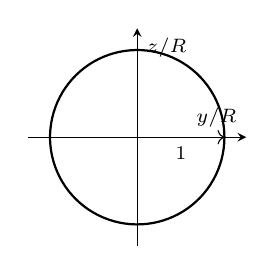
\begin{tikzpicture}
\begin{axis}[
    width=\linewidth,height=4.35cm,
    axis equal image,
    axis lines=center,
    xlabel={$y/R$},ylabel={$z/R$},
    xmin=-1.25,xmax=1.25,ymin=-1.25,ymax=1.25,
    ticks=none,
    clip=false,
    label style={font=\scriptsize},
]
\addplot[black,thick,domain=0:360,samples=100] ({cos(x)},{sin(x)});
\addplot[black,->] coordinates {(0,0) (1,0)} node[midway,below,font=\scriptsize] {$1$};
\end{axis}
\end{tikzpicture}

\small (b) Axial view: phase closure
\end{minipage}\hfill
\begin{minipage}[t]{0.32\textwidth}
\centering
\begin{tikzpicture}
\begin{axis}[
    width=\linewidth,height=4.35cm,
    axis lines=middle,
    xlabel={$x/R$},ylabel={$y/R$},
    xmin=0,xmax=3.8,ymin=-1.25,ymax=1.25,
    xtick={0,3.495},xticklabels={$0$,$2\pi q$},
    ytick={-1,0,1},
    tick label style={font=\scriptsize},
    label style={font=\scriptsize},
]
\addplot[black,thick,domain=0:3.495,samples=100] {cos(deg(x/0.55632418))};
\end{axis}
\end{tikzpicture}

\small (c) Side view: spatial periodicity
\end{minipage}
\caption{Three representations of the same local helical geometry, shown in units of the primitive radius $R$ with $q=a/R$. Over one transverse phase cycle, the axial coordinate advances by $2\pi a=2\pi qR$. The side projection is spatially periodic; it is not by itself a propagating wave.}
\label{fig:helix-projections}
\end{figure*}

It is equally important to state what the picture does \textbf{not} prove.

The relation \[
y=R\cos(x/a)
\] is a spatially periodic projection. It is not yet a propagating wave. A physical wave requires an additional time-evolution law, a dispersion relation, amplitude dynamics, superposition rules, and a relativistically consistent notion of transport.

Likewise, TEF does not presently derive \(c\) from the static helix. The requirement is instead that a completed rollout dynamics recover

\conceptbox{A common local causal structure with Lorentz-invariant signal propagation}

and no observable preferred source frame.

Electromagnetic radiation and photons belong to the same electromagnetic sector; gravitational radiation belongs to another. TEF's target is therefore not to explain several unrelated numerical coincidences of speed, but to seek a common lower-level realization of the relativistic causal structure already established by experiment.

\section{Matter, Motion, and Ordinary Gravity}\label{matter-motion-and-ordinary-gravity}

\subsection{Two-source rollout compatibility}\label{two-source-rollout-compatibility}

Consider two complete matter closures \(C_A\) and \(C_B\), with associated rollout structures \(S_A\) and \(S_B\).

TEF investigates gravity not as a primitive force acting across a background container, but as a compatibility problem of the jointly realized rollout geometry:

\[
\boxed{
S_A\leftrightarrow S_B.
}
\]

For an adapted local axis connecting two sources, the two outward rollout orientations oppose one another schematically, \[
A\longrightarrow\qquad\longleftarrow B.
\]

The intuition of partial cancellation may be useful in a weak-field picture, but ordinary vector subtraction in a pre-existing space is not taken as fundamental. The primitive object is the globally admissible geometry formed by the two rollout structures.

In a source/test-body limit, this picture should reduce to an effective description in which the dominant source determines the geometry and the weakly perturbing body follows that geometry. Any viable TEF completion must recover the empirical successes of general relativity in this limit.

\subsection{Rollout generation is not gravitational backreaction}\label{rollout-generation-is-not-gravitational-backreaction}

The strongest conceptual clarification developed in the present work is

\conceptbox{rollout generation $\neq$ gravitational backreaction}

A complete matter closure is provisionally assigned independent rollout-source identity.

A spacetime excitation is not.

But this does \textbf{not} mean that excitation energy, momentum, pressure, stress, motion, or interaction energy can be removed from gravitational physics.

Schematically,

\conceptbox{complete closure $\rightarrow$ independent rollout source}

while

\conceptbox{full energy--momentum state $\rightarrow$ effective geometric backreaction}



Figure~\ref{fig:source-backreaction} summarizes the distinction between independent rollout-source identity and gravitational backreaction.

\begin{figure*}[t]
\centering
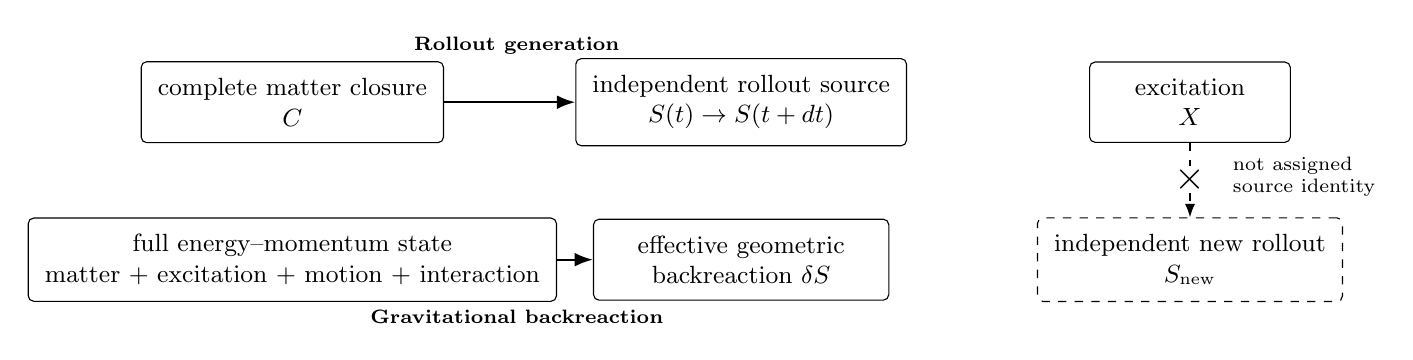
\begin{tikzpicture}[
    >=Latex,
    every node/.style={font=\small},
    box/.style={draw,rounded corners=2pt,align=center,inner sep=6pt,minimum height=1.02cm},
    soft/.style={draw,dashed,rounded corners=2pt,align=center,inner sep=6pt,minimum height=1.02cm}
]
\node[box,minimum width=3.25cm] (C) at (-5.7,1.0) {complete matter closure\\$C$};
\node[box,minimum width=4.05cm] (S) at (0.0,1.0) {independent rollout source\\$S(t)\rightarrow S(t+dt)$};
\node[box,minimum width=5.15cm] (T) at (-5.7,-1.0) {full energy--momentum state\\matter + excitation + motion + interaction};
\node[box,minimum width=3.75cm] (D) at (0.0,-1.0) {effective geometric\\backreaction $\delta S$};
\node[box,minimum width=2.55cm] (X) at (5.7,1.0) {excitation\\$X$};
\node[soft,minimum width=3.15cm] (SN) at (5.7,-1.0) {independent new rollout\\$S_{\rm new}$};

\node[font=\scriptsize\bfseries] at (-2.85,1.72) {Rollout generation};
\draw[->,thick] (C) -- (S);
\node[font=\scriptsize\bfseries] at (-2.85,-1.72) {Gravitational backreaction};
\draw[->,thick] (T) -- (D);
\draw[->,dashed] (X) -- (SN);
\node[font=\scriptsize,align=left] at (7.15,0.05) {not assigned\\source identity};
\node[font=\Large,fill=white,inner sep=0pt] at (5.7,0.02) {$\times$};
\end{tikzpicture}
\caption{Working distinction between rollout generation and gravitational backreaction. A globally complete matter closure is provisionally assigned independent rollout-source identity. The effective geometric response, by contrast, depends on the full energy--momentum state, including excitation, motion, and interaction contributions. Within the present working hypothesis, an excitation is not by itself assigned an independent new rollout source; if it later participates in forming a new globally complete closure, source identity is reassessed at that closure level.}
\label{fig:source-backreaction}
\end{figure*}

In a continuum limit, the conventional stress--energy tensor \(T_{\mu\nu}\) may therefore remain the correct effective bookkeeping object even if TEF assigns different microscopic ontology to the contributions entering it.

This distinction is intended to accommodate the observed gravitational role of photons, electrons, kinetic energy, field energy, and binding energy without declaring each of them an independent generator of a new spacetime rollout.

No backreaction law is derived here. Recovering the correct one is a central dynamical obligation.

\subsection{Motion remains an open problem}\label{motion-remains-an-open-problem}

A uniform boost of a complete closure should not redefine its intrinsic source label merely because a different observer assigns it a different energy.

The detailed relation among intrinsic closure state, four-momentum, motion-dependent energy, and effective gravitational response is therefore deliberately postponed.

This is not an appeal to the historical notion of ``relativistic mass.'' TEF must eventually reproduce the modern Lorentz-covariant energy--momentum structure. The present paper simply avoids using conventional mass as a primitive explanation of rollout.

\section{Spacetime Excitation: Photon, Electron, and Phase Transport}\label{spacetime-excitation-photon-electron-and-phase-transport}

\subsection{Excitations live on rollout; they do not create a second rollout}\label{excitations-live-on-rollout-they-do-not-create-a-second-rollout}

Let \(X\) denote a spacetime excitation.

The present hypothesis is

\[
\boxed{
X\not\rightarrow S_{\rm new}.
}
\]

Within the present working hypothesis, an excitation is not assigned an independent rollout-source identity.

Nevertheless, \[
X\rightarrow\delta S
\] is allowed as backreaction on the existing realized geometry.

An excitation may also exchange energy--momentum with a matter closure, changing the closure state and therefore its subsequent rollout: \[
X+C\rightarrow C'
\rightarrow S'(t+dt).
\]

This distinction preserves source identity while allowing physically required feedback.

\subsection{Photon and electron as different excitation classes}\label{photon-and-electron-as-different-excitation-classes}

A photon is explored as a rollout-synchronous electromagnetic excitation rather than as a miniature object moving through an ontologically separate spatial container.

The electron is explored as a persistent, phase-organized excitation state.

These are ontological hypotheses, not substitutes for QED. A successful TEF completion must still reproduce relativistic quantum dynamics, interference, polarization, spin, statistics, and measured scattering amplitudes.

\subsection{Rollout phase is a reference structure, not the whole quantum-state phase}\label{rollout-phase-is-a-reference-structure-not-the-whole-quantum-state-phase}

A simple scalar quantum state can be written as \[
\psi=\sqrt{\rho}\,e^{i\varphi}.
\]

Earlier TEF drafts risked identifying the full phase \(\varphi\) directly with a unique background rollout phase. That is too strong.

The weaker working picture is

\conceptbox{Rollout supplies a local phase reference and transport structure.}

while

\conceptbox{The excitation retains state-dependent relative phase and internal degrees of freedom.}

Schematically one may write, only as a local illustration, \[
\psi_X
=
\sqrt{\rho_X}\,
e^{i[\Theta_R+\varphi_X]},
\] where \(\Theta_R\) denotes a local rollout-phase reference and \(\varphi_X\) denotes excitation-dependent relative phase.

This decomposition is not claimed to be unique or fundamental. Its purpose is to prevent two different concepts from being collapsed into one.

Different states in the same spacetime can possess different momentum phases, interference phases, spinor components, and entanglement structure. Multi-particle states may live naturally in configuration space or Fock space rather than being reducible to one scalar amplitude on ordinary space. TEF must accommodate that standard quantum freedom.

\subsection{Density and current: a restricted illustration}\label{density-and-current-a-restricted-illustration}

For a low-energy single scalar excitation one may use \[
\rho=|\psi|^2
\] as a normalized density and write, schematically, \[
\int_\Sigma \rho\,d\mu_S=1.
\]

This is only an illustrative restricted limit.

State norm, conserved charge, conserved current, and particle number are not generally the same object. Relativistic electron dynamics requires a covariant current structure; photon localization and multi-excitation sectors require additional care; particle number need not be conserved in creation and annihilation processes.

TEF therefore does not promote \(\rho\) to a universal conserved ``amount of excitation.''

Likewise, the framework does not choose a quantum-measurement interpretation here. It requires only that any eventual theory reproduce definite localized measurement records, Born-rule statistics, Bell correlations, no-signalling, and the relevant conservation laws.

\subsection{Observable motion is transport, not arbitrary phase velocity}\label{observable-motion-is-transport-not-arbitrary-phase-velocity}

Overall phase evolution does not define a particle trajectory.

Observable electron motion must be associated with gauge-invariant transport of the excitation---such as an appropriate conserved current or wavepacket structure---not with an arbitrary overall phase or phase velocity.

In a free-particle or appropriate eikonal limit, phase derivatives encode the familiar canonical momentum and energy relations, \[
\mathbf p=\hbar\nabla\varphi,
\qquad
E=-\hbar\,\partial_t\varphi.
\]

In the presence of gauge coupling, observable transport instead requires the corresponding gauge-covariant combinations. With a conventional sign choice these take the schematic form \[
\boldsymbol\pi
=
\hbar\nabla\varphi-Q\mathbf A,
\qquad
\mathcal E_{\rm mech}
=
-\hbar\partial_t\varphi-QV,
\] where \(Q\) is the signed electric charge and \((V,\mathbf A)\) denotes the electromagnetic potential in the same convention. Here \(\mathcal E_{\rm mech}\) denotes the mechanical-energy combination obtained after removing the scalar-potential term; in a relativistic setting it may include rest energy and should not be read as nonrelativistic kinetic energy.

These expressions remain compatibility targets rather than a derived TEF quantum dynamics.

\section{Interaction Clues, Not a Completed Field Theory}\label{interaction-clues-not-a-completed-field-theory}

The present framework does not claim that the known interactions have already been derived from one helix. It records several structural clues that emerged independently in earlier TEF work.

\subsection{Strong sector: closure first}\label{strong-sector-closure-first}

The matter-topology branch suggests

\conceptbox{primitive strong-sector problem $\sim$ maintaining admissible global closure of incomplete matter sub-sectors}

Quark-like pieces may be locally persistent while globally incomplete. Rerouting or switching structure is then required to maintain or change an admissible closure.

This does not derive QCD gluons, color dynamics, or confinement. It identifies a structural problem that a future strong-sector energy functional must solve.

Residual nuclear interaction between already complete hadron-level closures must ultimately emerge from the same completed strong theory; it is not licensed as an unrelated extra rule.

\subsection{Weak sector: interface conjecture with limited scope}\label{weak-sector-interface-conjecture-with-limited-scope}

Earlier TEF matter-topology work suggests that a process which changes local matter class may involve reconfiguration of the boundary between closed matter structure and open rollout modes.

The present statement is therefore deliberately limited:

\conceptbox{Matter-changing weak processes are candidate closure--rollout interface processes.}

This is not yet a universal definition of the weak interaction.

Purely leptonic weak processes provide an immediate pressure test because they need not contain a hadron-like closed matter source. A future interface theory must either extend naturally to such processes or the conjecture must be revised.

\subsection{Electromagnetism: covariant phase transport}\label{electromagnetism-covariant-phase-transport}

Absolute rollout phase is not taken to be directly observable. Physical phase comparison requires transport between local frames.

Schematically, \[
\Delta\varphi_{\rm phys}
=
\varphi_B-\varphi_A-\int_\gamma \mathcal A.
\]

Under a local phase change, \[
\varphi\rightarrow\varphi+\alpha,
\] the connection conventionally transforms as \[
\mathcal A\rightarrow\mathcal A+d\alpha
\] for this sign convention, so the transported comparison remains invariant modulo \(2\pi\).

This makes a gauge-like connection a natural object to investigate.

Connection, holonomy, and geometric phase are already standard tools in gauge and quantum theory. As one recent example, non-perturbative QED has been studied using a \(U(1)\) Berry connection and associated holonomy over gauge-configuration space \cite{Gamboa2025}. That construction is not the TEF proposal and does not derive electromagnetic coupling from rollout; it is cited only to place phase-transport language in an established mathematical-physics context.

However, a nontrivial electromagnetic field cannot be obtained merely by renaming \[
\mathcal A=d\Theta_R
\] for one smooth single-valued scalar phase, because such a pure gradient has vanishing local curvature. A viable TEF electromagnetic construction therefore requires independent connection freedom, nontrivial patching, or another structure capable of producing nonzero curvature.

If \(\mathcal A\) is eventually identified with the physical electromagnetic potential, its charge normalization, units, representations, and field strength must all be derived consistently.

\subsection{A local helical-frame clue}\label{a-local-helical-frame-clue}

A local helix carries three natural adapted directions: \[
\mathbf e_r,\qquad
\mathbf e_\phi,\qquad
\mathbf e_x.
\]

This motivates a candidate primitive picture in which radial response is compared with electrostatic behavior, azimuthal phase rotation with magnetic behavior, and axial rollout compatibility with ordinary gravity.

Symbolically, \[
E_r,\qquad B_\phi,\qquad G_x
\] are useful \textbf{local prototype configurations}.

They are not universal restrictions on observable fields.

A general electromagnetic configuration need not possess one common helix axis; a static electric field does not automatically require a nonzero magnetic component; and general gravity includes tidal and tensor structure that cannot be reduced to one spatial direction.

The purpose of the adapted-frame picture is therefore heuristic and constructive: it proposes simple local seeds from which a covariant field theory might be built and tested.

\subsection{Charge and spin remain open constructions}\label{charge-and-spin-remain-open-constructions}

Electric charge \(Q\) is provisionally treated as a discrete excitation-topology label or representation property that determines coupling to the phase-transport connection.

The exact invariant is unknown.

Positive and negative charge may be represented by conjugate excitation classes, \[
X_- = X_+^*,
\] but this is not yet a derivation of charge quantization.

Likewise, a framed helix can be lifted from \[
SO(3)
\] to \[
Spin(3)\simeq SU(2),
\] making \(4\pi\) restoration mathematically available. This establishes spinorial compatibility, not a derivation of electron spin-\(1/2\) or Fermi statistics.

\section{A Separate Energetic Calibration Conjecture}\label{a-separate-energetic-calibration-conjecture}

The preceding ontology does not depend logically on the empirical relation discussed in this section.

Let \[
E_e=0.51099895069(16)\ {\rm MeV}
\] denote the measured electron rest-energy scale in conventional notation, and define \[
E_I=(\sqrt2G_F)^{-1/2},
\] with \[
G_F=1.1663787(6)\times10^{-5}\ {\rm GeV}^{-2}.
\]

Then \[
E_I\simeq246.21965\ {\rm GeV}.
\]

The conjectured bridge is \[
\boxed{
E_C^2=\frac{\pi}{2}E_eE_I.
}
\]

Equivalently, \[
E_e=\frac{2}{\pi}\frac{E_C^2}{E_I}.
\]

Using the stated inputs gives \[
E_C=444.56094\ {\rm MeV}.
\]

The coefficient \(2/\pi\) already appears in the frozen Paper-I helix condition \[
q\sqrt{1+q^2}=\frac{2}{\pi},
\] but that fact does not derive its placement in the energy relation above. The energy mapping is an additional conjecture.

The relation is therefore frozen as a modular calibration hypothesis rather than presented as a consequence of the rollout ontology.

\subsection{Retrospective QCD comparison}\label{retrospective-qcd-comparison}

Bulava \emph{et al.} \cite{Bulava2024} reported \[
\sqrt{\sigma}
=
445(3)_{\rm stat}(6)_{\rm sys}\ {\rm MeV}
\] for a flux-tube branch parameter in a coupled static-source analysis including string breaking and extrapolation to physical light-quark mass.

The numerical proximity to \[
E_C=444.56094\ {\rm MeV}
\] is worth recording.

Its evidential status is limited.

The QCD benchmark was already known during development of the relation, so the comparison is retrospective rather than a blind prediction. The quoted \(\sigma\) is a parameter of the flux-tube branch in the coupled-channel description, not a universal nonzero asymptotic slope of the complete full-QCD ground-state potential. The cited result was also obtained at a single lattice spacing rather than through a continuum-limit determination.

A more recent lattice study at physical quark masses directly examined the chromo-electric flux-tube profile and reported hints of string breaking at a source separation in the range \[
0.963\ {\rm fm}\lesssim d^*\lesssim1.156\ {\rm fm}
\] \cite{Cea2026}. This does not validate the TEF closure picture, but it reinforces the need to distinguish a pre-breaking flux-tube branch from any supposed universal asymptotic linear potential in full QCD.

The comparison target should therefore be frozen narrowly: a future improved determination of the same long-distance flux-tube branch scale should test the conjecture. The target should not be replaced after the fact by whichever QCD quantity lies closest.

\subsection{Global rollout bookkeeping scale}\label{global-rollout-bookkeeping-scale}

Earlier TEF work introduced \[
E_S=\frac{c^4}{G}P_1,
\qquad
P_1=\pi q\ell_P,
\] giving \[
E_S=\pi qE_P
\sim2.1\times10^{19}\ {\rm GeV}.
\]

This remains a global rollout bookkeeping scale associated with one primitive cycle. It is not interpreted here as a local extractable energy packet, an energy assigned to each microscopic line, or a quantity already connected dynamically to the low-energy bridge.

The relation between \(E_S\) and observable lower-energy sectors remains open.

\section{What Is Actually Frozen?}\label{what-is-actually-frozen}

This paper freezes a \textbf{working research baseline}, not a completed physical theory.

The present baseline consists of the following limited commitments:

\begin{enumerate}
\def\labelenumi{\arabic{enumi}.}
\tightlist
\item
  Persistent matter is associated with dynamically admissible global closure.
\item
  Only a globally complete level is provisionally assigned independent rollout-source identity.
\item
  Rollout is a continuing update of spacetime structure rather than dilution into a pre-existing spatial volume.
\item
  Within the present working hypothesis, spacetime excitation is not assigned an independent rollout-source identity.
\item
  Excitation energy, momentum, stress, motion, and interaction energy must nevertheless participate in effective gravitational backreaction.
\item
  The helical geometry supplies phase-bearing local structure and spatial periodicity, but not by itself a propagating wave equation.
\item
  A completed dynamics must recover local Lorentz invariance and the common relativistic causal structure.
\item
  Rollout may supply a local phase reference and transport connection, while excitations retain state-dependent phase and internal quantum degrees of freedom.
\item
  Strong-sector closure, matter-changing weak interface processes, electromagnetic phase transport, and axial rollout compatibility are research directions rather than completed interaction laws.
\item
  \(\Phi_R(C)\) is only an as-yet undefined intrinsic rollout-source label.
\item
  The deeper substrate beneath matter, rollout, and excitation remains outside TEF's modeled ontology, while observable closure formation, destruction, and source update remain within the programme's obligations.
\item
  The \(444.56\ {\rm MeV}\) energy bridge is an independent, replaceable calibration conjecture.
\end{enumerate}

Several ideas are intentionally \textbf{not} frozen:

\begin{itemize}
\tightlist
\item
  the microscopic location from which a complete closure rolls out spacetime;
\item
  a specific universal electric/radial, magnetic/azimuthal, gravitational/axial field law;
\item
  a universal identification of all weak interaction with closed-matter interface dynamics;
\item
  a universal scalar excitation density;
\item
  a completed charge topology;
\item
  a spin derivation;
\item
  black-hole or singular-limit ontology;
\item
  a law relating motion-dependent energy to rollout generation;
\item
  a dynamical relation between the global scale \(E_S\) and low-energy physics.
\end{itemize}

\section{The Next Mathematical Problems}\label{the-next-mathematical-problems}

The framework should now become narrower rather than broader.

The next progress should come from solving explicit constructions.

\subsection{Emergent metric and weak-field gravity}\label{emergent-metric-and-weak-field-gravity}

Starting from a conserved or otherwise well-defined intrinsic source structure, TEF must derive an effective metric or equivalent observable geometry without first assuming the Euclidean area law it seeks to explain.

The resulting two-source limit must reproduce at least the weak-field inverse-square regime, universal free fall, redshift, and the relevant post-Newtonian structure.

\subsection{Lorentz-covariant rollout dynamics}\label{lorentz-covariant-rollout-dynamics}

The local helix and source-attached language must not generate an observable preferred frame.

A successful model must show how the same microscopic structure yields Lorentz-consistent propagation and four-momentum transformation.

\subsection{Excitation transport}\label{excitation-transport}

A concrete excitation equation must distinguish rollout reference phase from state-dependent quantum phase and reproduce a conserved relativistic current in the appropriate limit.

This is the natural place to test the electron hypothesis against Schrödinger, Dirac, and field-theoretic descriptions.

\subsection{Gauge connection}\label{gauge-connection}

If electromagnetic coupling is related to phase transport, TEF must construct a genuine connection with nonzero curvature and derive its normalization, charge representations, Maxwell limit, and Lorentz transformation properties.

\subsection{Closure energetics}\label{closure-energetics}

The strong-sector programme must continue from topology to an energy functional. The key test is whether maintaining an admissible closure under separation or deformation produces a constrained energy law resembling the established confining regime without contradicting string breaking and QCD gauge structure.

\subsection{Matter-changing interface dynamics}\label{matter-changing-interface-dynamics}

The weak-sector conjecture must be tested first on a concrete process. Beta decay remains a natural case because it explicitly changes local matter class while coupling to leptonic modes.

The same construction must then confront purely leptonic weak processes. If it cannot, the interface interpretation is incomplete.

\subsection{Independent empirical output}\label{independent-empirical-output}

The energetic bridge is retrospective. The programme therefore needs a second quantitative relation fixed before comparison with its target data.

Without that step, numerical correspondence remains suggestive rather than predictive.

\section{Discussion}\label{discussion}

The central idea of TEF is not that every known interaction has already been reduced to a helix.

It is that a useful division may exist between \textbf{geometry of open rollout}, \textbf{topology of persistent matter}, and \textbf{excitation of the realized spacetime structure}.

That division was not present clearly at the beginning of the programme. It emerged gradually.

The early helical work treated spacetime geometry as the main object. The matter-topology work then showed that forcing matter to be a literal copy of the open helix was unnecessary and possibly misleading. Closure and relative framing became the more natural language for matter. The interface branch then asked how the two descriptions could meet.

The present paper adds one further clarification: the identity of a rollout source need not be the same thing as the source of gravitational backreaction.

This allows a complete matter closure to play a special role in generating or updating spacetime while photons, electrons, motion, and interaction energy still influence the effective geometry.

The same caution applies to quantum phase. Rollout may provide phase-bearing geometry and a transport reference without monopolizing the state-dependent phase of every quantum excitation.

These distinctions make the framework less visually simple than saying ``everything is one helix.'' They also make it substantially more compatible with the structures that a viable theory must reproduce.

The programme should therefore resist adding further correspondences until one of the current ones becomes a genuine dynamical construction.

\section{Conclusion}\label{conclusion}

The Emergent Frame asks whether the physical frame associated with matter may itself be emergent.

The present working answer begins with three modeled categories: persistent closed matter topology, spacetime rollout, and spacetime excitation. A deeper substrate is acknowledged as a possible common origin but is not modeled.

Globally complete matter closures are provisionally assigned independent rollout-source identity. Rollout is treated as an ongoing update of spacetime structure rather than emission into a pre-existing Euclidean container. The inherited helical geometry provides a phase-bearing local model in which transverse phase closes while axial rollout continues, but a propagation law remains to be derived.

Within the present working hypothesis, spacetime excitations are not assigned independent rollout-source identity. They nevertheless carry energy and momentum and must contribute to the effective gravitational response. Rollout generation and gravitational backreaction are therefore distinct.

Photon and electron phenomena are investigated as different excitation classes. Rollout may supply local phase reference and transport structure, but quantum excitations retain state-dependent relative phase and internal degrees of freedom. No universal scalar excitation density, measurement ontology, charge topology, or spin derivation is claimed.

The interaction programme remains modular. Strong-sector research concerns closure energetics; matter-changing weak processes motivate a closure--rollout interface conjecture; electromagnetic research concerns covariant phase transport; and ordinary gravity concerns compatibility of matter-generated rollouts. Radial, azimuthal, and axial helix directions remain candidate local prototype configurations, not universal field directions.

An intrinsic rollout-source label \[
\Phi_R(C)
\] is introduced only as a placeholder for a future source law. Conventional mass is not used as a primitive concept.

Finally, \[
E_C^2=\frac{\pi}{2}E_eE_I
\] is retained as a separate retrospective calibration conjecture whose future value depends on frozen-target testing, not on reinterpretation after new data appear.

The immediate research task is therefore clear: stop expanding the ontology and solve one of its missing equations.

\balance

\begin{thebibliography}{99}
\small
\bibitem{Einstein1905}
A. Einstein, ``Zur Elektrodynamik bewegter K{\"o}rper,'' \emph{Annalen der Physik} \textbf{17}, 891--921 (1905).

\bibitem{deBroglie1924}
L. de Broglie, \emph{Recherches sur la th{\'e}orie des quanta}, doctoral thesis, University of Paris (1924).

\bibitem{Feynman1948}
R. P. Feynman, ``Space-Time Approach to Non-Relativistic Quantum Mechanics,'' \emph{Reviews of Modern Physics} \textbf{20}, 367--387 (1948).

\bibitem{CODATA2025}
P. J. Mohr, D. B. Newell, B. N. Taylor, and E. Tiesinga, ``CODATA recommended values of the fundamental physical constants: 2022,'' \emph{Journal of Physical and Chemical Reference Data} \textbf{54}, 033105 (2025). \href{https://doi.org/10.1063/5.0279860}{doi:10.1063/5.0279860}.

\bibitem{Bulava2024}
J. Bulava, F. Knechtli, V. Koch, C. Morningstar, and M. Peardon, ``The quark-mass dependence of the potential energy between static colour sources in the QCD vacuum with light and strange quarks,'' \emph{Physics Letters B} \textbf{854}, 138754 (2024). \href{https://doi.org/10.1016/j.physletb.2024.138754}{doi:10.1016/j.physletb.2024.138754}.

\bibitem{WuPaperI}
X. Wu, ``A Helical Spacetime Ansatz Linking the Planck Scale and Electroweak Mixing,'' Version 5.1 (2026), Zenodo. \href{https://doi.org/10.5281/zenodo.22101000}{doi:10.5281/zenodo.22101000}.

\bibitem{WuPaperII}
X. Wu, ``From a Gravity-Calibrated Helix to a Conditional Fine-Structure Correspondence,'' Version 4.7 (2026), Zenodo. \href{https://doi.org/10.5281/zenodo.22117153}{doi:10.5281/zenodo.22117153}.

\bibitem{WuPaperIII}
X. Wu, ``From a Gravity-Calibrated Helix to Neutrino Oscillation Correspondences: A Third Cross-Sector Comparison of the Frozen TEF Shape Parameter,'' Version 4.2 (2026), Zenodo. \href{https://doi.org/10.5281/zenodo.22150998}{doi:10.5281/zenodo.22150998}.

\bibitem{WuPaperIV}
X. Wu, ``Closed Matter and Open Space: A Relative-Framing Ansatz for Incomplete Quark Sectors and the Matter--Space Interface,'' Version 4.6 (2026), Zenodo. \href{https://doi.org/10.5281/zenodo.22256714}{doi:10.5281/zenodo.22256714}.

\bibitem{WuPaperV}
X. Wu, ``From a Gravity-Calibrated Helix to a Strong-Interaction Confinement Correspondence,'' Version 4.1 (2026), Zenodo. \href{https://doi.org/10.5281/zenodo.22412464}{doi:10.5281/zenodo.22412464}.

\bibitem{WuPaperVI}
X. Wu, ``From a Gravity-Calibrated Helix to a Matter--Spacetime Interface: Closure Obstruction and a Factorized Mass-Squared Ansatz,'' Version 3.2 (2026), Zenodo. \href{https://doi.org/10.5281/zenodo.22649267}{doi:10.5281/zenodo.22649267}.

\bibitem{Jacobson1995}
T. Jacobson, ``Thermodynamics of Spacetime: The Einstein Equation of State,'' \emph{Physical Review Letters} \textbf{75}, 1260--1263 (1995). \href{https://doi.org/10.1103/PhysRevLett.75.1260}{doi:10.1103/PhysRevLett.75.1260}.

\bibitem{Wetterich2004}
C. Wetterich, ``Gravity from Spinors,'' \emph{Physical Review D} \textbf{70}, 105004 (2004). \href{https://doi.org/10.1103/PhysRevD.70.105004}{doi:10.1103/PhysRevD.70.105004}.

\bibitem{FischerPaganini2026}
P. Fischer and C. F. Paganini, ``Causal fermion systems: spacetime as the web of correlations of a many-body quantum system,'' \emph{Classical and Quantum Gravity} \textbf{43}, 045005 (2026). \href{https://doi.org/10.1088/1361-6382/ae2379}{doi:10.1088/1361-6382/ae2379}.

\bibitem{Gamboa2025}
J. Gamboa, ``Berry Phase in Non-Perturbative QED,'' arXiv:2503.24194 [hep-th] (2025).

\bibitem{Cea2026}
P. Cea, V. Chelnokov, L. Cosmai, and A. Papa, ``Hints for string breaking in QCD,'' arXiv:2607.07143 [hep-lat] (2026).
\end{thebibliography}

\end{document}
